\documentclass{article}
\usepackage[top=2.5cm,bottom=1.5cm,inner=3cm,outer=3cm,includehead,includefoot]{geometry}
\usepackage[nottoc,numbib]{tocbibind}
%\usepackage{fancyhdr}
%\usepackage{hyperref}
%\usepackage{setspace}
\usepackage{graphicx}

\pagestyle{fancy}
\lhead{R\&D project proposal}
\rhead{\thepage}
\renewcommand{\baselinestretch}{1.5} 
\cfoot{}
\renewcommand{\headrulewidth}{0.6pt}
\renewcommand{\footrulewidth}{0.6pt}
\title{\Large{R\&D Project Proposal}\\
\vspace{0.8cm}
\textbf{Evaluation of Semantic Textual Similarity Approaches for Automatic Short Answer Grading}\\
[15mm]}
\author{\makebox[.9\textwidth]{\textbf{Ramesh Kumar}}\\
[10mm]
 \and First Advisor:\\
 [2mm]\textbf{Prof. Dr. Paul Pl\"oger} \and Second Advisor:\\
  [2mm]\textbf{M.Sc. Deebul Nair}\\
  [30mm] }

\date{Master of Autonomous Systems  \\ 
[2mm]
University of Applied Sciences Bonn-Rhein-Sieg \\
[25mm]
\today}
\begin{document}
\maketitle
\thispagestyle{empty}
\newpage
\section*{Abstract}

Semantic textual similarity computes the equivalence of two sentences on the basis of its conceptual similarity. It is widely used in natural language processing tasks such as question answering, essay scoring, machine translation, text classification, and information extraction. This research and development project focuses on one of the application of semantic textual similarity; automatic short answer grading. Automatic short answer grading system automatically assigns a grade to a response provided by a student by comparing with one or more model answers. The task is to evaluate the existing semantic similarity techniques for automatic short answer grading  on publicly available datasets and on datasets created from in-house exams. All techniques will be examined based on performance, reliability, amount of human effort required, ease of implementation, and response rate.

\newpage
\section{Introduction}

Semantic textual similarity measures the equivalence of words or sentences in terms of meaning.	
This similarity can range from exactly identical to completely unrelated. Similarity score is generated on a certain scale to represent distance between words or sentences, higher the score the more similar the meaning of the two sentences or two words is. There is difference between semantic similarity and semantic relatedness. Semantic similarity considers only ``is a'' relations, while semantic relatedness consider any relation between two terms. Example: ``car'' is similar to ``truck'' or ``bus'', but it is also related to ``road'' and ``driving'' \cite{similarity}. In other words, semantic similarity is a subset of semantic relatedness.


Semantic similarity measures are classified into three major types: 
	\subsection{String-based Similarity}
	String-based similarity computes similarity between two text strings based on string matching regardless of their meaning. Most widely known algorithm for string similarity is Levenshtien Distance\cite{wikiString}. It determines the similarity based on  minimum number of operations(addition, substitution, deletion) to transform one string into another. The other approaches are Hamming distance, Damerau-Levenshtein distance,
Needleman-Wunsch distance, Smith-Waterman distance,
Jaro Winkler distance, Dice’s coefficient, Jaccard similarity and longest common substring\cite{survey}.
	
	
\subsection{Corpus-based Similarity}
	
	 Corpus-based similarity measures degree of similarity between words using information acquired from large corpora such as Wikipedia, Google, AltaVista and many more.
These measures are unsupervised and are used to compare the relatedness of words in corpora without prior knowledge of their meaning or usage. Words are compared with respect to context in which they occur. These measures can be used to compare various units of language; from words to texts. However, limitations are; words that are compared must occur at least few times, and it is difficult to compute the semantic similarity rather than semantic relatedness as words are compared with respect to context \cite{corpusbased}. 
Corpus based measures includes latent semantic analysis, explicit semantic analysis, normalized google distance, Hyperspace analogue to language, and Distributionally similar words using co-occurances(DISCO)\cite{survey}.

\subsection{Knowledge-based Similarity}


Knowledge-based similarity determines the degree of  similarity by using information derived from semantic networks. One of the most popular semantic network is WordNet, which is a lexical database for the English language. It categorize the words of language as a set of synonyms, called synsets. Along with this, it also includes definition and examples of how to use them. In other words, WordNet can be considered as a combination of dictionary and thesaurus\cite{wordNet}. Knowledge-based approaches are categorized into two sub-groups: 
\begin{itemize}
\item \textbf{Measures of Semantic Similarity}
	\begin{itemize}
	\item These measures include ``is a'' relations between two words such as ``is a kind of'' and ``is a part of''.  There are six measures of semantic similarity, based on information content and path length\cite{survey}:
	\begin{itemize}
	\item \textbf{Information Content:}
	
	\begin{itemize}
			
	\item Resnik(res)
	\item Lin(lin)
	\item Jiang and Conrath(jcn)
	
	\end{itemize}
	\end{itemize}
	%% path length
	\begin{itemize}
	\item \textbf{Path Length:}
	\begin{itemize}
	
	
	\item Leacock and Chodorow(lch)
	\item Wu \& Palmer(wup)
	\item Path
	\end{itemize}
\end{itemize} 
	\end{itemize}
\end{itemize}

\begin{itemize}
\item \textbf{Measures of Semantic Relatedness}
	\begin{itemize}
	\item These measures include general relation between two words such as "car" and "road" are related to each other. There are three measures of semantic relatedness; Hirst and St-Onge(hso), Lesk(lesk), and vector pairs(vector)\cite{survey}.
	\end{itemize}
\end{itemize}

Semantic similarity is useful in many applications such as question answering, essay scoring, machine translation, text classification, information extraction and so on.

However, this research and development project focuses on automatic short answer grading. The task is to evaluate the existing semantic similarity techniques for automate short answer grading on previously existing datasets and on new datasets that will be generated based on in-house exams. Following section briefly gives description of Automatic Short Answer Grading system and data sets that will be used for this task.
\subsection{Automatic Short Answer Grading:}
Automatic short answer grading is a system that automatically assign grade to answers provided by student. The length of answer consist of approximately two or three sentences.  Many approaches do not consider the grammar and coherency in answer, while, main concern is to grade the response by comparing with model answer provided by instructor. To compute the similarity between two sentences, features are extracted from sentences and based on evaluation metrics such as Pearson correlation, root mean square error etcetera, similarity score is computed and assigned to student answer. To automate short answer grading, many techniques such as Ontology, Semantic similarity matching and Statistical methods are used\cite{ASAG}. Automatic grading is preferred over manual grading to save time, avoid bias errors and save expenses. Along with this, system can also provide grade to the students immediately after submission of answers.

\subsection{Data Sets} 


The data sets for this task will be kaggle\cite{kaggle}, Texas \cite{texas}, and SemEval'13 task 7 competition. The brief description of each database is given below:
	\begin{itemize}
	
	
	\item \textbf{Kaggle}
		\begin{itemize}
		\item The data set for short answer grading was used for competition organized by William and Flora Hewlett Foundation(Hewlett Foundation). During this competition, ten data sets were used. The average length of selected responses were around 50 words. All answers were written from students of Grade 10, and were double-scored by human graders using integer scale from 0 to 3. All the data sets were consisted of different training size.   
		\end{itemize}
	\item \textbf{Texas}
		\begin{itemize}
		\item The data set for short answer grading is used in \cite{texas}. This data set was created from Data Structures course at the University of North Texas. It consist of ten assignments and two examinations, overall 80 questions. The total number of answers including all the students were 2273. These answers were used to train the perceptron. Furthermore, answers were independently graded by two human graders using integer scale from 0 to 5, where 0 represent completely incorrect and 5 represent perfect answer. Moreover, average grade of two evaluators was taken and used as the gold standard to examine the automatic grading task.
		\end{itemize}
		
	\item \textbf{SemEval 2013(Semantic Evaluation)}
		\begin{itemize}
		\item Semantic Evaluation is an ongoing series of evaluations to evaluate semantic analysis systems\cite{semWiki}. SemEval 2013 data set was part of semantic evaluation workshop in 2013. The task introduced two data sets; BEETLE and SCIENTSBANK. The SCIENTSBANK training corpus consist of approximately 10,000 responses for 197 questions from 15 different science domains. Furthermore, responses were graded by multiple human graders on a scale of "Correct", "Partially correct incomplete", "Contradictory", "Irrelevant" and "non domain"\cite{iterative}. On the other hand, BEETLE training corpus contain 56 questions from the basic electricity and electronics domain, and approximately 3000 student answers of 56 questions. Each answer is approximately of 1 or 2 sentences. Furthermore, second manual annotation pass was carried out on a set of questions to check for consistency.\cite{semEval2013}
		\end{itemize}



 Furthermore, in order to evaluate the approaches, existing approaches use evaluation metrics such as Pearson correlation coefficient Pearson correlation coefficient, root mean square, mean quadratic weighted kappa, F1 score and many more. Following section briefly describe evaluation metrics.   	

\begin{itemize}

%%%%%%%%% Evlaution %%%%
\item \textbf{Evaluation Metrics}
	\begin{itemize}
	\item This section briefly describes metrics that can be used to evaluate the existing approaches.
	\end{itemize}

	\begin{itemize}
	\item \textbf{Mean Quadratic Weighted Kappa}
		\begin{itemize}
		\item This is a scoring metric, it measures closeness between scores of human grader and scores of automatic short answer grader. Furthermore, it varies between 0 and 1, where 0 represent scores are completely dissimilar and 1 represent exact agreement.\cite{kappa}
		\end{itemize}
	\item \textbf{F1 score}
		\begin{itemize}
		\item It is an accuracy metric, used to measure the performance of word segmentation, part of speech(POS) tagging and dependency parsing\cite{NLPUnderstanding}. Furthermore, word segmentation is to divide the string of characters into its component words and part of speech (pos) tagging is to determine the part of speech of a particular word in the text. While, dependency parsing analyses the grammatical structure of a sentence in the text \cite{dependencyParser}. F1 score ranges from 0 to 1, where 1 represents best score and 0 represents worst score. 
		\end{itemize}
	\item \textbf{Pearson Correlation Coefficient}
		\begin{itemize}
		\item It is another metric used to measure similarity between the terms. It measures how two terms are related to each other. It has a value between +1 and -1, where +1 represent terms are completely similar and -1 represent terms are completely dissimilar.\cite{wikiPearson}
		\end{itemize}
	\item \textbf{Root Mean Square Error (RMSE)}
		\begin{itemize}
		\item It is square root of the mean/average of the square of all the error. It is used to compute the error between the terms. Higher error represent terms are not similar. As compare to mean absolute error, this metric amplifies and severely punishes large errors.\cite{kaggleroot}
		\end{itemize}
	\end{itemize}
	\end{itemize}
\end{itemize}

%%%% evaluation metrics completed %%%%%%%
\newpage
\section{Problem Addressed}
\begin{itemize}
\item This work will focus on surveying existing approaches of semantic similarity for short answer grading.
\item The existing approaches will be evaluated on available datasets such as Kaggle, Texas, SemEval 2013, and also on dataset created from in-house exams. %based on performance, reliability, dataset used for training and user-friendly environment. 
\item All techniques will be examined based on performance, reliability, amount of human effort required, ease of implementation, and response rate.
\end{itemize}

 	 
\newpage
\section{State of the art}

Semantic similarity measures are divided into three types:
\subsection{String Based Similarity}
\centering
\begin{figure}[h]
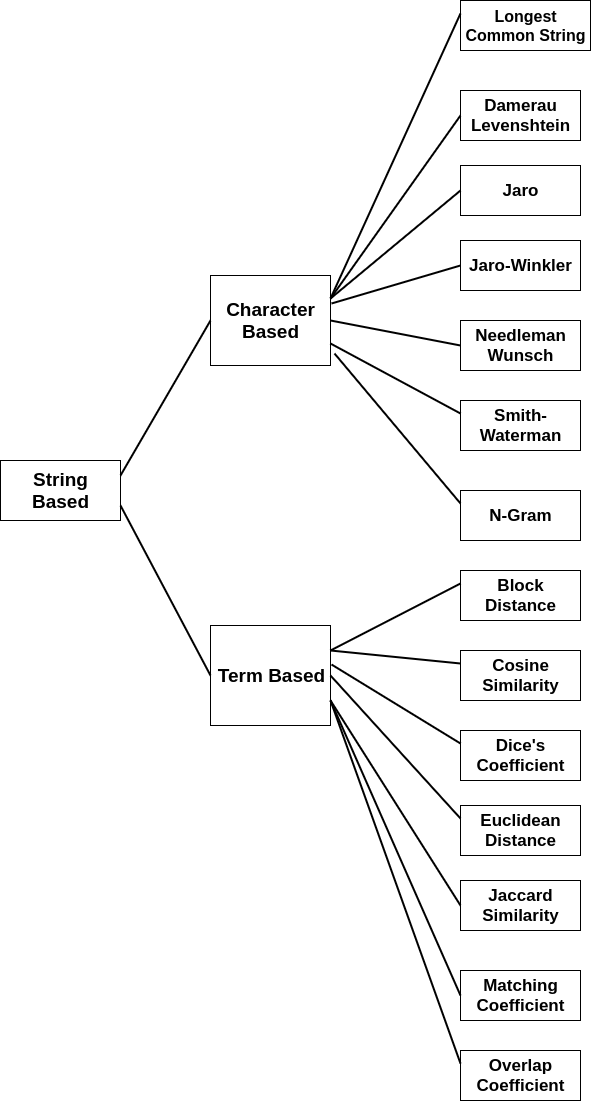
\includegraphics[width=10cm,height=12cm]{string_similarity.png}
\caption{String-Based Similarity Measures\cite{survey}}
\end{figure}
\begin{flushleft}
String-based similarity determines similarity or dissimilarity of two strings in the text. Following section briefly describes related work in String-based similarity: 
\end{flushleft}

\begin{itemize}
\item In \cite{jaccard}, authors introduced  a measure of Jaccard similarity with Prolog programming language to determine similarity of words in the data sets. Furthermore, dataset is prepared from set of words; mainly concerned with agriculture domain. On the other hand, information that is not correct contains grammatical mistakes, misspelled words, crashed words and over-typed words. Similarity between words is computed by using Jaccard coefficient. Performance of similarity is evaluated by using the precision, recall and F-measure. Lastly, authors concluded that, Jaccard similarity perform well in computing the similarity score, but it fails to detect the over-typed words in the data sets. 
\item In \cite{ldistance}, authors proposed the Levenshtein distance technique to improve the Dictionary lookup methods. Dictionary lookup methods take string as input and compute the similarity with strings in the dictionary. Furthermore, similarity between strings is computed based on Levenshtein distance, where distance is computed based on number of deletions, insertions, or substitutions required to transform one string into another. In order to improve the dictionary lookup method, authors modify the algorithm of existing approaches by incorporating different method to compute weight between strings. Lastly, authors concluded that, current approach improve the performances of dictionary lookup methods. However, this approach is applied to words having length from three to five, but words with more lengths were yet to be verified.  
\end{itemize}
\newpage
\begin{flushleft}
\subsection{Corpus Based Similarity}
\end{flushleft}
\begin{center}
\begin{figure}[h]
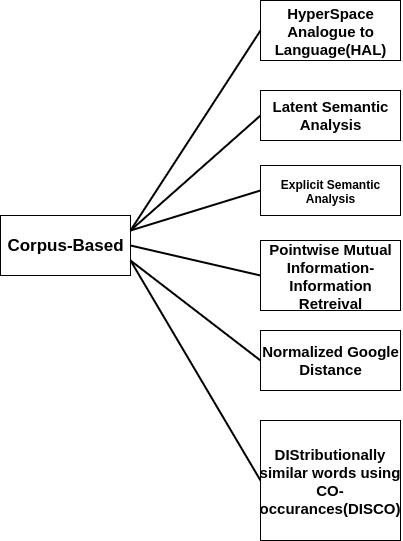
\includegraphics[width=10cm,height=6.5cm]{corpus_similarity.png}
\caption{Corpus-Based Similarity Measures\cite{survey}}
\end{figure}
\end{center}
\begin{flushleft}
It is a semantic similarity measure that compute similarity or dissimilarity of sentences or words based on information gained from large corpora. Following section briefly describes related work in Corpus-based similarity: 
\end{flushleft}

\begin{itemize}
\item In \cite{lsa}, author introduced system for semantic similarity of documents using Latent Semantic Analysis(LSA). LSA is statistical method that is used to extract the relationships into word passages. In the paper, dataset is consist of ten PDF documents from Medline Industries on different topics. The collection of text or corpus was transformed into term-document matrix; size of 338*10. Furthermore, corpus was pre-processed and singular value decomposition(svd) is applied to reduce the dimension of corpus. To determine the closeness between the terms, cosine similarity is computed. Moreover, by observing the results, authors concluded that LSA is able to deduce the conceptual meaning of terms and associate the meaning with other terms. However, in general, LSA cannot handle polysemy(words with more than one meaning) effectively, therefore, corpus used for this approach did not have terms that have same meaning.
%% PMI %%%
\item In \cite{PMI}, author proposed PointWise Mutual Information(PMI) and Information Retreival(IR) algorithm to solve task of recognizing synonyms, given a problem word and a set of alternative words. In order to evaluate the algorithm, author used 80 synonym test questions from the Test of English as a Foreign Language(TOEFL) and 50 synonym test questions from a collection of tests for students of English as a Second Language(ESL). Furthermore, this paper also compared results of PMI-IR algorithm with Latent Semantic Analysis(LSA), where PMI-IR outperforms the LSA with score 10\% higher than LSA. Furthermore, it is concluded that, to implement this algorithm, for certain applications there is requirement of very high speed system as network access time for querying large Web pages can be more. Along with this, this algorithm can achieve better results when size of corpus is smaller.    
\end{itemize}
\begin{flushleft}
\subsection{Knowledge Based Similarity}
\end{flushleft}

\centering
\begin{figure}[h]
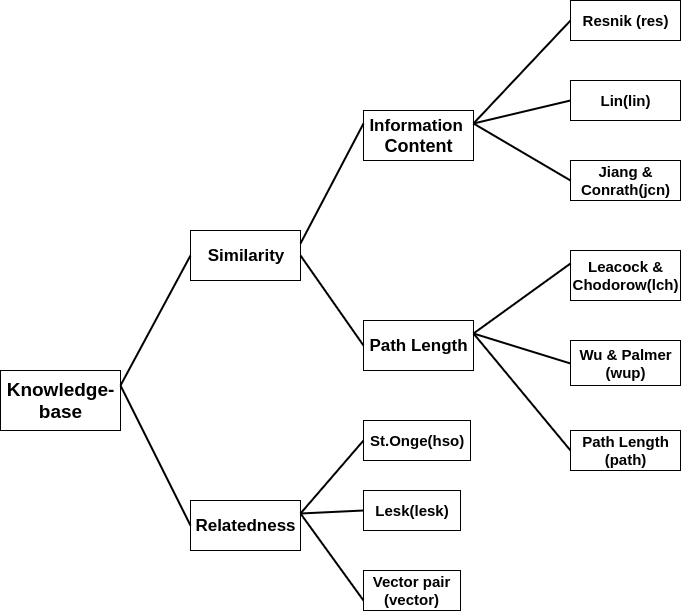
\includegraphics[width=12cm,height = 10cm]{knowledge_base.png}
\caption{Knowledge-Based Similarity Measures\cite{survey}}
\end{figure}
\begin{itemize}
\item In \cite{lch}, Leacock \& Chodorow(lch) presented the statistical classifier that identifies the sense of word whether it is noun, verb, adjective or adverb in the context of sentence by combining topical context with local cues. To train the general text corpus, knowledge base of WordNet's lexical relation was used. Furthermore, authors identified that identification of word sense in local context is superior as compare to topical context when statistical classifier is being used. To evaluate the approach, test results are compared with the manually tagged training examples. While, to determine word sense in a non-topical context is yet to be done.
%%% lin
\item In \cite{lin}, Lin presented the algorithm that computes the similarity measures in general domain rather than specific domain in terms of information theory. Previous approaches such as distance-based measures assume that domain is specific rather than general. To compute the similarity, this approach uses Resnik's measure\cite{resnik} of similarity and augments the normalization factor of two input concepts in the information content. Furthermore, results of current algorithm are compared in applications of different domains, where different similarity measures have been implemented.
\end{itemize}

\newpage
\begin{flushleft}
Different systems have been developed in order to automate short-answer grading. This section show some of the most relevant works previously done in this field.
\end{flushleft}


\begin{itemize}
\item In \cite{text-similarity}, authors  explored and evaluated unsupervised techniques for short-answer grading system. The paper has established three valuable contributions, firstly, authors have shown comparison of performance between corpus based and knowledge based measures.
Secondly, authors examined the effect of domain and corpus size on the performance of corpus-based measures. As a result, authors concluded that notable improvement can be achieved with the use of medium size domain-specific corpus built from Wikipedia. 
Thirdly, using the method similar to pseudo-relevance feedback technique, system is able to improve the quality by considering the students correct response.  
\end{itemize}

\begin{itemize}
\item In \cite{MdArfat}, another automatic short answer grading system is presented. The system implemented text-similarity features with key grading-specific constructs that extended state-of-the-art systems developed for text-similarity. Furthermore, authors computed similarity features from the text such as: text similarity, question demoting, term weighting and length ratio. By extracting these features from the text, authors shown that proposed system has a high accuracy, simple design and fast runtime.  
\end{itemize}

\begin{itemize}
\item In \cite{texas}, authors evaluated the existing bag-of-word approaches to assess the short text responses. Furthermore, to improve the performance of previously existing approaches, authors used machine learning techniques such as support vector machine to combine lexical semantic similarity with graph alignment features. To comprehend the syntactic differences between sentences, rudimentary dependency-graph alignment module is implemented, where dependency graph of student's response is aligned with the instructor's model answer. Moreover, final grades are assigned to the student's response by comparing the Pearson's correlation coefficient of system and human graders. To evaluate the approach, authors created the dataset named as Texas, consists of 2273 student answers from the computer science assignments. As a result, it is concluded that machine learning techniques improve the performance of existing bag-of-word approaches. While, rudimentary alignment features are not enough to be considered as  standalone grading system. For the future work, quality of answer alignments can be enhanced by training a model using graph-graph alignments.  
\end{itemize}
\newpage
\section{Expected Results}

\begin{itemize}

\item \textbf{Minimum:}
	 \begin{itemize}
	 \item Survey the existing semantic similarity approaches for short answer grading.
	 \item Review existing datasets for short answer grading.
	 \item Create in-house datasets.	 
	 \end{itemize}
\item \textbf{Expected:}
	 \begin{itemize}
	 \item Evaluate selected semantic similarity measures on existing automatic short answer grading datasets.
   %	 \item Evaluate existing databases based on performance, reliability, human-effort, and response rate using same databases.
	 \item Evaluate use cases by including students response.
	 \item Integrate all the evaluated methods with nbgrader.
	 
	 \end{itemize}
\item \textbf{Maximum:}
	 \begin{itemize}
	 \item Implement one method for short answer grading in a development server
	 \end{itemize}
\end{itemize}
\newpage
\section{Work Plan}

\subsection{Gantt Chart}
\centering
\begin{figure}[h]
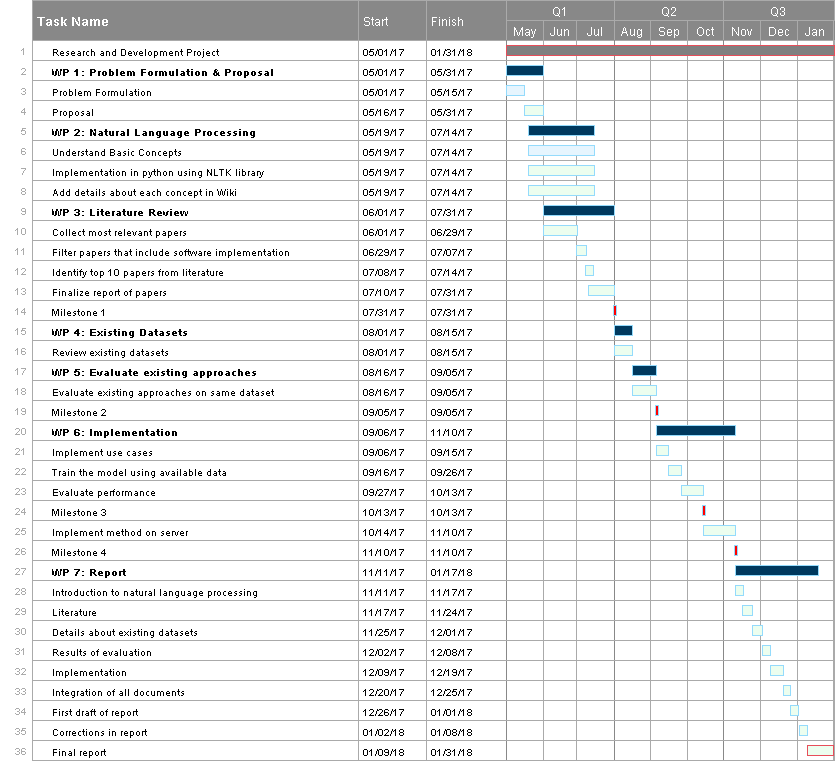
\includegraphics[width=15cm,height=15cm]{workplan.png}
\end{figure}
\newpage
\begin{thebibliography}{9}

\bibitem{similarity}

https://en.wikipedia.org/wiki/Semantic\_similarity

\bibitem{wikiString}

https://en.wikipedia.org/wiki/String\_metric

\bibitem{corpusbased}

Sébastien Harispe, Sylvie Ranwez, and Stefan Janaqi, ``Semantic Similarity from Natural Language and Ontology Analysis'' 

\bibitem{survey}
Wael H. Gomaa and Aly A. Fahmy, ``A Survey of Text Similarity Approaches'', International Journal of Computer Applications (0975 – 8887) Volume 68 No.13, April 2013

\bibitem{wordNet}
https://en.wikipedia.org/wiki/WordNet

\bibitem{kaggle}
https://www.kaggle.com/c/asap-sas/data

\bibitem{texas}
Mohler, Michael and Bunescu, Razvan and Mihalcea, Rada, ``Learning to Grade Short Answer Questions Using Semantic Similarity Measures and Dependency Graph Alignments'', Proceedings of the 49th Annual Meeting of the Association for Computational Linguistics: Human Language Technologies - Volume 1, 2011

\bibitem{semWiki}

https://en.wikipedia.org/wiki/SemEval

\bibitem{iterative}
Shourya Roy, Himanshu S. Bhatt, and Y. Narahari ``An Iterative Transfer Learning Based Ensemble Technique for Automatic Short Answer Grading'', CoRR, 2016

\bibitem{ASAG}
 P. Selvi and A. K. Banerjee, ``Automatic ShortAnswer Grading System
(ASAGS)'', Inter JRI Computer Science and Networking 2(1), pp.19–23, 2010.

\bibitem{semEval2013}
Myroslava O. Dzikovska, Rodney D. Nielsen, Chris Brew, Claudia Leacock, Danilo Giampiccolo, Luisa Bentivogli, Peter Clark, Ido Dagan, and Hoa Trang Dang, "SemEval-2013 Task 7: The Joint Student Response Analysis and 8th
Recognizing Textual Entailment Challenge", 

\bibitem{kappa}

Dan Preston and Danny Goodman, "Automated Essay Scoring and The Repair of Electronics", http://snap.stanford.edu/class/cs341-2012/reports/03-Preston\_cs341\_\-\_Dan\_and\_Danny\_\-\_Final.pdf

\bibitem{NLPUnderstanding}
Chin-Yew Lin, Nianwen Xue, Dongyan Zhao, Xuanjing Huang, and Yansong Feng, ``Natural Language Understanding and Intelligent Applications: 5th CCF Conference on Natural Language Processing and Chinese Computing'', NLPCC 2016, and 24th International Conference on Computer Processing of Oriental Languages, ICCPOL 2016, Kunming, China, December 2–6, 2016,


\bibitem{dependencyParser}
https://nlp.stanford.edu/software/nndep.shtml
\bibitem{wikiPearson}

https://en.wikipedia.org/wiki/Pearson\_correlation\_coefficient

\bibitem{kaggleroot}

https://www.kaggle.com/wiki/RootMeanSquaredError

\bibitem{jaccard}
Suphakit Niwattanakul, Jatsada Singthongchai, Ekkachai Naenudorn and Supachanun Wanapu,``Using of Jaccard Coefficient for Keywords
Similarity'',Proceedings of the International Multi-Conference of Engineers and Computer Scientists 2013 Vol I,
IMECS 2013, March 13 - 15, 2013, Hong Kong

\bibitem{ldistance}
Rishin Haldar and Debajyoti Mukhopadhyay, ``Levenshtein Distance Technique in Dictionary Lookup
Methods: An Improved Approach'',CoRR,2011
\bibitem{lsa}
Chelsea Boling,``Semantic Similarity of Documents Using Latent Semantic Analysis'', Proceedings of the National Conference On Undergraduate Research (NCUR) 2014 University of Kentucky, Lexington, KY April 3-5, 2014

\bibitem{PMI}
Turney, P. 2001. ``Mining the web for synonyms: PMI-IR versus
LSA on TOEFL'', In Proceedings of the Twelfth European Conference
on Machine Learning (ECML-2001).

\bibitem{lch}
Leacock, C., Chodorow, M., and George A.,  ``Combining local context and WordNet sense similarity for word sense identification''. In WordNet, An Electronic Lexical Database. The MIT Press, 1998.

\bibitem{lin}
Lin, D., ``An information-theoretic definition of similarity'',
In Proceedings of the International Conference on Machine Learning,1998

\bibitem{resnik}
Resnik Philip, ``Using information content to evaluate semantic similarity'', In Proceedings of the 14th International Joint Conference
on Artificial Intelligence,1995

\bibitem{peter}
Peter Kolb, ``Experiments on the difference between semantic
similarity and relatedness'', Proceedings of the 17th Nordic Conference of Computational Linguistics NODALIDA 2009, 4, page 81--88. Northern European Association for Language Technology, (2009)
\bibitem{randomwalk}
Daniel Ramage, Anna N. Rafferty, and Christopher D. Manning, ``Random Walks for Text Semantic Similarity'', Proceedings of the 2009 Workshop on Graph-based Methods for Natural Language Processing

\bibitem{evaluationOfsemanticApproaches}
Slimani Thabet, ``Description and Evaluation of Semantic Similarity Measures Approaches'', International Journal of Computer Applications, 2013
\bibitem{MdArfat} 
Md Arafat Sultan, Cristobal Salazar, Tamara Sumner, ``Fast and Easy Short Answer Grading with High Accuracy'' ,NAACL HLT 2016, The 2016 Conference of the North American Chapter of the Association for Computational Linguistics: Human Language Technologies, San Diego California, USA, June 12-17, 2016, 2016, 1070-1075

\bibitem{Automated-AssessmentofShortFree-TextResponses} 
R. Siddiqi and C. J. Harrison, ``On the Automated Assessment of Short
Free-Text Responses'',  pp. 1–11, 2008

\bibitem{text-similarity}
Mohler, Michael and Mihalcea, Rada, ``Text-to-text Semantic Similarity for Automatic Short Answer Grading'', Proceedings of the 12th Conference of the European Chapter of the Association for Computational Linguistics,2009 

%\bibitem{c-rater}
%Sukkarieh, Jana Zuheir and Blackmore, John, ``C-rater: Automatic Content Scoring for Short Constructed Responses'', Proceedings of the Twenty-Second International FLAIRS Conference (2009)



\end{thebibliography}
\end{document}